\documentclass{scrartcl}

\usepackage[ngerman]{babel}
\usepackage{fontspec}

% some useful packages
\usepackage{mathtools}
\usepackage{amssymb}
\usepackage{graphicx}
\usepackage[printwatermark]{xwatermark}
%\usepackage{hyperref}
%wird eh durch error durch default ersetzt -> auskommeentiert
%\hypersetup{%
%	pdfborder={0 0 0}
%}
\usepackage{titlesec}

\newwatermark*[pages=16-20,color=gray!75,angle=45,scale=3,xpos=0,ypos=0]{DRAFT}
\newcommand{\sectionbreak}{\clearpage}

\input{commands}

\setmainfont{SourceSerifPro-Regular.otf}[
    BoldFont		=	SourceSerifPro-Bold.otf,
    ItalicFont		=	EBGaramond08-Italic.otf]

\begin{document}
	\setlength{\parindent}{0pt}

	\begin{titlepage}

		%Title
		\begin{center}
			\huge \bfseries Chrono Command \\
			\large  Web Basierte Zeiterfassung
		\end{center}

		%Subtitle
		\begin{center}
				\large Pflichtenheft \\
		\end{center}

		%Authors
		\begin{center}
			Jannis Friedmann \\
			David Kuhmann \\
			Maria Schmid \\
			Xiaoming Wang \\
			Jan Zenkner \\

		\end{center}

		%Date
		\begin{center}
			\large \today
		\end{center}
	
		\vfill
	\end{titlepage}
	\thispagestyle{empty}

	\pagenumbering{roman}

	\clearpage
	\pagestyle{empty}
	\tableofcontents

	\clearpage
	\pagestyle{plain}
	\pagenumbering{arabic}
	\setcounter{page}{1}

	\section{Einleitung}

Dieses Dokument beschreibt die Qualitätssicherungsphase des PSE-Projektes \linebreak \emph{ChronoCommand}. Die Qualitätssicherung soll die Qualität des Produktes feststellen, ob der Code korrekt und stabil ist, Fehler finden und diese anschließend beheben.
\\\\
Die Qualitätssicherung umfasst folgende Punkte:
\begin{itemize}
	\item \textbf{Testszenarien}
\end{itemize}
Bei den Testszenarien werden die Testfälle aus dem Pflichtenheft am laufenden Programm getestet. Dabei soll eine grobe Übersicht über die Funktionalität der Software entstehen.

\begin{itemize}
	\item \textbf{Testabdeckung}
\end{itemize}
Für die Qualitätssicherungsphase üblichen Tests, gibt die Testabdeckung einen Überblick. Es wurde versucht eine hohe Abdeckung zu erreichen, um möglichst viele Fehler zu finden.

\begin{itemize}
	\item \textbf{Fehlerbeschreibung}
\end{itemize}
Alle, in den vorherigen Punkten, gefundenen Fehler und deren Behebung sind in der Fehlerbeschreibung beschrieben. 

	\section{Zielbestimmung}

\subsection{Musskriterien}

\begin{itemize}
	\item Starten und Stoppen von einer Zeiterfassung
	\item Zeiten sind nachträglich erfassbar
	\item Zeiten sind nachträglich änderbar
	\item erfasste Zeiten können Tätigkeiten zugeordnet werden
	\item erfasste Zeiten können Kategorien zugeordnet werden
	\item Warnungen wenn Zeiten nicht eingetragen sind
	\item Möglichkeit die erfassten Zeiten an den Admin zu übersenden
	\item Warnungen wenn gesetzlich Pausen genommen werden müssen
	\item Warnungen wenn zu erfasster Zeit keine Tätigkeit zugeordnet ist
	\item Warnungen wenn zu erfasster Zeit keine Kategorie zugeordnet ist
	\item Vergangene Zeiten sind einsehbar
	\item Hinzufügen von Accounts
	\item Löschen von Accounts
	\item Ändern von Accounts
	\item Bestimmte Benutzer sind Administratoren
	\item Bestimmte Benutzer sind Betreuer
	\item Administratoren legen fest welche Benutzer von welchem Betreuer betreut werden
	\item Backups werden regelmäßig angefertigt
	\item Es kann zwischen LDAP und lokalen Accounts zur Benutzerverwaltung gewählt werden
	\item Zeiten sollen durch eine graphische Übersicht visulisiert werden (Heatmap, Punch Card) TODO überprüfen
\end{itemize}


\subsection{Wunschkriterien}

\begin{itemize}
	\item Mehrere Frontendimplementierungen sind möglich
	\item Zeitvorhersagen anhand vergangener Arbeitszeit
	\item Überwachung der Arbeitszeit auch ohne abgebene Zeiten möglich
	\item Erfassung der Tätigkeiten während der Arbeitszeit
	\item Möglichkeit die IP-Range, von der aus sich Administrator einloggen können, beschränken
	\item Kalendarische Übersicht an erfasster Zeit
	\item Zeiten sollen durch eine graphische Übersicht visulisiert werden TODO auf aktualität überprüfen
	\item Über eine Toolbar Zeit erfassen und eine Tätigkeit zuordnen
\end{itemize}


\subsection{Abgrenzungskriterien}
\begin{itemize}
	\item Korrekter Ablauf im Internet Explorer wird nicht unterstüzt
	\item Die Nutzung der gleichen Instanz durch mehrere Firmen und die damit erforderliche Trennung der Daten wird nicht unterstützt
	\item Es wird nur auf Einhaltung der deutschen Gesetzgebung geachtet
\end{itemize}

	\section{Produkteinsatz}
Das System dient zur Verwaltung und Kontrolle der Arbeitszeiten von Mitarbeitern* (Studierende), Analyse verschiedener Projekte anhand der erfassten \emph{Zeiten} und der entsprechenden \emph{Tätigkeiten}.
Die von \emph{Benutzern*} angegebenen Daten werden auf einem Server gespeichert. Auf dem Server gespeicherte Daten können mit einem Internet Browser aufgerufen, tabellarisch und grafisch dargestellt werden.
Durch Nachrichtenfunktionen soll der Kontakt zwischen \emph{Benutzern*}, \emph{Betreuern*} und \emph{Administratoren*} sichergestellt werden.
Des Weiteren gibt es eine Benutzerverwaltung, um die Zugriffsrechte auf die Daten zu verwalten.
\subsection{Anwendungsbereiche}
\begin{itemize}
	\item Der Anwendungsbereich umfasst sämtliche gewerbliche Betriebsumfelder sowie Universitäten, Institutionen, Vereine,
	welche die Arbeitszeiten von Studierenden oder ähnlichen Mitarbeitern* auf effizienter Weise verwalten wollen. Die Anzahl der Studierenden bzw. Mitarbeitern* sind normalerweise groß.
\end{itemize}

\subsection{Zielgruppen}
\begin{itemize}
	\item Die Anwender in den Zielgruppen sind \emph{Benutzer*}, \emph{Betreuer*} und \emph{Administratoren}*.
	Die Zielgruppen haben ein gruppeneigenes Berechtigungsprofil, das auf die Benutzerbedürfnisse zugeschnitten ist und nur Zugriff auf die nötigen Funktionen erlaubt.
	Dabei hat der \emph{Benutzer*} nur Zugriffsberechtigung auf seine eigenen Daten, während der \emph{Betreuer*} auf alle seinen zugewiesenen \emph{Benutzer*} und der \emph{Administrator*} auf alle Daten Zugriff hat.
\end{itemize}

\subsection{Betriebsbedingungen}
\begin{itemize}
	\item Die Betriebsbedingungen müssen für die Anwendung auf einem zentralen Webserver spezifiziert werden. Der Server läuft im Dauerbetrieb und unbeaufsichtigt.
	Client-User brauchen einen normalen Internetfähigen Rechner oder Smartphone.
\end{itemize}

	\section{Produktumgebung}

\subsection{Software Backend}
\begin{itemize}
    \item Als Basis des Backends dient Java 8.
    \item Das erstellen der benötigten Dateien übernimmt Maven.
\end{itemize}

\subsection{Software Middleware}
\begin{itemize}
    \item Die Schnittstelle zwischen Backend und Frontend wird durch REST implemetiert.
\end{itemize}

\subsection{Software Frontend}
\begin{itemize}
    \item Die Weboberfläche basiert auf HTML5 und wird mithilfe von VAADIN aus Java Code generiert.
\end{itemize}

\subsection{Hardware User}
    Da die Anwendung auf einer Web-Oberfläche läuft ist, muss die Hardware einen Webbrowser besitzen der HTML5 und JavaScript unterstützt.

\subsection{Hardware Server}
    Der Server muss Java 8 installiert haben.
    Außerdem wird ein Java Servlet Webserver benötigt.


	\section{Funktionale Anforderungen}

Die den Wunschkriterien zugeordneten Anforderungen sind mit einem "`+"' hinter der Indentifikationsnummer markiert.

\subsection{Stundenzettel und Zeiterfassung}

\begin{requirements}
    \req[Zeiterfassung]{F110}
    Ein User kann in seiner Hauptseite eine Zeiterfassung starten und stoppen.
    \begin{requirements}
        \req[Kategorie]{F111} Eine Zeiterfassung ist mit einer Kategorie versehen.
        \req[Tätigkeit]{F112} Eine Zeiterfassung ist mit einer Tätigkeit verbunden.
        \req[Zeiterfassung ändern]{F113} Eine Zeiterfassung kann nachträglich geändert werden.
        \req[Alternative Zeiterfassung]{F114} Eine Zeiterfassung kann auch manuell ohne das Starten und Stoppen einer Zeit erfasst werden.
        \req[Zeiterfassung löschen]{F115} Eine erfasste Zeit kann vom Benutzer wieder gelöscht werden.
    \end{requirements}

    \req[Gesetzliche Vorgaben]{F120}
    Die Zeiterfassung und der Stundenzettel folgen den gesetzlichen Bestimmungen.
    \begin{requirements}
        \req[Maximale Arbeitszeit]{F121} Die gesetzlich maximale Arbeitszeit kann bei einer Zeiterfassung nicht überschritten werden (siehe §3 ArbZG).
        \req[Pausenzeiten]{F122} Eine Zeiterfassung kann nicht dem Stundenzettel hinzugefügt werden wenn für ihren Umfang gesetzliche Pausenzeiten nicht eingetragen wurden (siehe §4 ArbZG).
        \req[Ruhezeiten]{F123} Die Einhaltung der Ruhezeiten wird erzwungen (siehe §5 ArbZG).
        \req[Nachtarbeit]{F124} Administratoren können Nachtarbeit für einzelne Nutzer erlauben, allen anderen Nutzern ist Nachtarbeit nicht gestattet (siehe §6 ArbZG).
        \req[Sonn- und Feiertage]{F125} Die Einhaltung der Sonn- und Feiertagsruhe wird erzwungen (siehe §9 ArbZG).
		Dabei werden nur die Feiertage in Baden-Württemberg beachtet.
                Die Sonn- und Feiertagsruhe kann für einzelne Benutzer von Administratoren deaktiviert werden (siehe §10 ArbZG), dabei wird dann §11 ArbZG beachtet.
        \req[Manipulation verhindern]{F126} Die gesetzlichen Vorgaben sind über eine Konfigurationsdatei anpassbar deren Prüfsumme im Code hinterlegt ist.
                Daher muss zum Ändern der gesetzlichen Vorgaben das Programm neu compiliert werden.
    \end{requirements}

    \req[Stundenzettel]{F130}
    Der Stundenzettel stellt eine Aufzeichnung der Arbeitstunden in einem vorgesetzten Zeitraum dar.
    \begin{requirements}
        \req[Sichtbarkeit]{F131} Der Betreuer und der Administrator können den Stundenzettel einsehen.
        \req[Stundenzettel abgeben]{F132} Ist der Benutzer mit seiner Zeiterfassung in einem Zeitraum fertig, so kann er den Stundenzettel abgeben.
        \req[abgegebener Stundenzettel]{F133} Ein abgegebener Stundenzettel kann vom Benutzer nichtmehr verändert werden.
        \req[abgegebene Stundenzettel]{F134} Der Betreuer und der Admin werden über abgegebene Stundenzettel informiert
        \req[Stundenkonto]{F135} Im Stundenzettel ist die tatsächliche und die zu leistende Arbeitszeit sichtbar.
        \req[Betreuerkontrolle]{F136} Ein Stundenzettel kann vom Betreuer als Okay befunden werden.
        \req[Betreuerkontrolle erfolgreich]{F137} Ein vom Betreuer als Okay befundener Stundenzettel wird dem Admin als abgegeben angezeigt.
        \req[Betreuerkontrolle fehlgeschlagen]{F138} Ein vom Betreuer abgelehnter Stundenzettel wird als nicht abgegeben markiert, vom Betreuer kommentiert, und der Benutzer darüber informiert.
        \req[Stundenzettel exportieren]{F139} Ein Administrator kann alle abgegebenen Stundenzettel eines Monats zum Drucken exportieren.
        \req[Drucken]{F13A}Benutzer, Betreuer und Admins können Stundenzettel drucken.
    \end{requirements}

\end{requirements}

\subsection{Benutzer und Rechte}

\begin{requirements}
    \req[Benutzer]{F210}
    Ein Benutzer stellt den Standart User dar.
    \begin{requirements}
        \req[Stundenzettel]{F211} Ein Benutzer kann nur seinen eigenen Stundenzettel einsehen und verändern.
        \req[Warnungen]{F212} Ein Benutzer erhält nur Warnungen über seine eigenen Aktionen.
        \req[Erinnerungen]{F213} Ein Benutzer erhält nur Erinnerungen, die ihn selbst betreffen.
    \end{requirements}

    \req[Betreuer]{F220}
        Ein Betreuer ist für mehrere Benutzer zuständig.
        \begin{requirements}
            \req[Benutzer zuweisen]{F221} Einem Betreuer können Benutzer zugewiesen werden
            \req[Stundenzettel]{F222} Der Betreuer kann über seine Übersicht alle ihm zugewiesenen Benutzer einsehen
            \req[Warnungen]{F223} Der Betreuer erhält Warnungen für alle Benutzer die ihn zugewiesen sind.
            \req[Erinnerungen]{F224} Der Betreuer erhält Erinnerungen für alle Benutzer die ihm zugewiesen sind.
            \req[Stundenzettel prüfen]{F225} Der Betreuer überprüft die abgegebenen Stundenzettel der im zugewiesenen Benutzer.
        \end{requirements}

    \req[Admin]{F230}
        Ein Admin stellt das Verwaltungsorgan dar.
        \begin{requirements}
            \req[Benutzer erstellen]{F231} Der Admin kann neue Benutzer anlegen.
            \req[Benutzer editieren]{F232} Der Admin kann die Daten existierender Benutzer verändern.
            \req[Benutzer löschen]{F233} Der Admin kann einen existierenden Benutzer löschen.
            \req[Benutzer zuweisen]{F234} Der Admin kann Benutzer einem Betreuer zuweisen.
            \req[Betreuer Ansicht]{F235} Der Admin kann für jedes Team auch auf die Betrueransicht zugreifen.
        \end{requirements}
\end{requirements}

\subsection{Zeitüberwachung und Darstellung}
    \begin{requirements}
        \req[Graphische Darstellung Zeit]{F310+}
        \begin{requirements}
            \req[Übersicht Teams]{F311} Der Admin soll die bisher benötigte Zeit aller Teams auf seiner Hauptseite einsehen können.
            \req[Übersicht Betreuer]{F312} Dem Betreuer soll die bisher benötigte Zeit aller im zugewiesenen Benutzer angezeigt werden.
            \req[Übersicht Benutzer]{F313} Der Benutzer soll seine bisher aufgewedete Zeit graphisch angezeigt werden.
            \req[Burn Rate Benutzer]{F314} Der Benutzer soll seine durchschnittliche wöchentliche Stundenrate angezeigt bekommen.
        \end{requirements}

        \req[Graphische Darstellung Stundenzettelabgabe]{F320}
        \begin{requirements}
            \req[Übersicht Teams]{F321} Der Admin soll auf seiner Hauptseite die bisherigen Abageben von Stundenzetteln angezeigt bekommen.
            \req[Übersicht Betreuer]{F322} Der Betreuer soll den bisherigen Abgabefortschritt seines Teams dargestellt bekommen.
        \end{requirements}

        \req[Darstellung von Daten]{F330}
        \begin{requirements}
            \req[Heatmap]{F331} Benutzer können einsehen an welchen Tagen die meinste Arbeitszeit geloggt wurde.
            \req[Punch Card]{F332} Benutzer können einsehen zu welchen Zeiten die meinste Arbeitszeit geloggt wurde.
        \end{requirements}

        \req[Tätigkeiten Darstellung]{F340}
        \begin{requirements}
            \req[Tätigkeiten Ranking]{F341} Benutzer können sich den Zeitverbrauch pro Tätigkeit, gesammlt über alle Benutzer, anzeigen lassen.
            \req[Tätigkeits Heatmap]{F342} Benutzer können sich eine Tätigkeits Heatmap, anzeigen lassen.
        \end{requirements}
        
        \req[Übersicht aller Daten]{F350}
        \begin{requirements}
             \req[Admin]{F351} Admins können alle geleisteten Stunden aller HiWis graphisch einsehen.
             \req[Filter]{F352} Die graphische Anzeige erlaubt es nach Projekten, Betreuern, HiWis und Datum zu filtrieren.
        \end{requirements}

       \req[Framework zur Darstellung]{F360} Daten werden durch ein Statistik Framework visualisiert angezeigt.
    \end{requirements}

\subsection{Sonstige FA}
    \begin{requirements}
        \req[Sicherheit von Konfigurationen]{F410} Konfigurationsdateien sind durch einen Hash vor dem Editieren geschützt
        \req[Sicherheit der Datenbank]{F420} Die Datenbank wird durch einen Hash vor externem Editieren geschützt
        \begin{requirements}
            \req[Externe Veränderung der Datenbank]{F421} Sollte eine Veränderung stattgefunden haben, werden alle Nutzer über dieses externe Event informiert.
        \end{requirements}
    \end{requirements}


	\section{Produktdaten}

\subsection{Benutzerdaten}
\begin{requirements}
	\req [Benutzer] {D10}
	\begin{requirements}
		\req{D11} ID
		\req{D12} Name
		\req{D13} Vorname
		\req{D14} Email
		\req{D15} Passwort
		\req{D16} Rechte
		\req{D17} \em Zeiterfassungen \em
		\req{D18} \em Betreuer \em
	\end{requirements}
\end{requirements}

\subsection{Zeitdaten}
\begin{requirements}
	\req [Zeiterfassung] {D20}
	\begin{requirements}
		\req{D21} \em Benutzer \em  ID
		\req{D22} \em Kategorie \em
		\req{D23} \em Tätigkeit \em
		\req{D24} Beginn
		\req{D25} Ende
	\end{requirements}

	\req [Stundenzettel] {D30}
	\begin{requirements}
		\req{D31} \em Benutzer \em  ID
		\req{D32} \em Zeiterfassungen \em
		\req{D33} Stundenkonto
		\req{D34} Abgeschlossen
		\req{D35} \em Betreuer \em  geprüft
	\end{requirements}
\end{requirements}



	\section{Nichtfunktionale Anforderungen}

\subsection{Allgemeine Ziele}
\begin{requirements}
    \req{NF110} Die Navigation durch das \em{Frontend} ist Intuitiv.
\end{requirements}

\subsection{Benutzbarkeit, Performance und Stabilität}
\begin{requirements}
    \req{NF220} Die Ladezeit des \em{Frontends} liegt bei guter Internetverbindung unter 30 Sekunden.
    \req{NF230} Es wird auf Einblendungen, die die Benutzung des \em{Frontends} einschränken verzichtet.
    \req{NF240} Das \em{Frontend} läuft stabil, das bedeutet:
     \begin{itemize}
        \item Das \em{Frontend} verhält sich zu jedem Zeitpunkt vorhersehbar.
        \item Alle Zustände und Übergänge sind zu jedem Zeitpunkt definiert
        \item unerwartete Eingaben werden abgefangen.
        \item Im Ein-Benutzer Betrieb ist das \em{Frontend} stabil (Eine Zeiterfassung pro Nutzer).
     \end{itemize}
     \req{NF250} Das \em{Backend} läuft stabil, das bedeutet:
          \begin{itemize}
             \item Das \em{Backend} verhält sich zu jedem Zeitpunkt vorhersehbar.
             \item Alle Zustände und übergänge sind zu jedem Zeitpunkt definiert
             \item unerwartete Eingaben werden abgefangen.
             \item Das \em{Backend} verhält sich in folgenden Grenzen stabil:
	         \begin{itemize}
                    \item Es werden höchtens 25 gleichzeitige Anfragen an das \em{Backend} gestellt.
             \end{itemize}
          \end{itemize}
\end{requirements}

\subsection{Modularisierung in der Entwicklung}

\begin{requirements}
    \req{NF300} Um die Entwicklung und die Wartbarkeit des Produktes zu unterstützen, wird das Produkt in Module unterteilt.
    \begin{requirements}
        \req{NF310} Die Datenbank wird nicht Modularisiert.
        \req{NF320} Das \em{Backend} wird in folgende Module unterteilt:
            \begin{itemize}
                \item TODO
            \end{itemize}
        \req{NF330} Das \em{Frontend} wird in folgende Module unterteilt:
            \begin{itemize}
                \item Zeitmessung
                \item Benachrichtigungen
                \item Kalender
                \item Statistiken
                \item Stundenzettel Kern
            \end{itemize}
    \end{requirements}
\end{requirements}

\subsection{Qualität und Rechtliches}
\begin{requirements}
    \req{NF410} Die in Laufe des Projekts erstelle Artefakte sind gut
    \begin{itemize}
        \item zu warten (Einhaltung von Code Standarts).
        \item zu erweitern (Objektorientierter, modularer Aufbau.)
        \item dokumentiert.
        \item mit Testfällen abgedeckt (Unittests, Überdeckung > 75\%).
    \end{itemize}
    \req{NF420} Eine kommerzielle Veröffentlichung des Produkts ist möglich, u.a. gilt:
    \begin{itemize}
        \item benutzte Assets und Bibliotheken sind kommerziell nutzbar.
    	\item es finden sich Hinweise auf die jeweiligen Urheber und Lizenzen im Programm.
    \end{itemize}
    \req{NF430} \em{Datenbankelemente} liegen mindestens in der dritten Normalform vor.
\end{requirements}

	\section{Globale Testfälle}

\subsection{Funktionssequenzen}

	\section{Systemmodelle}

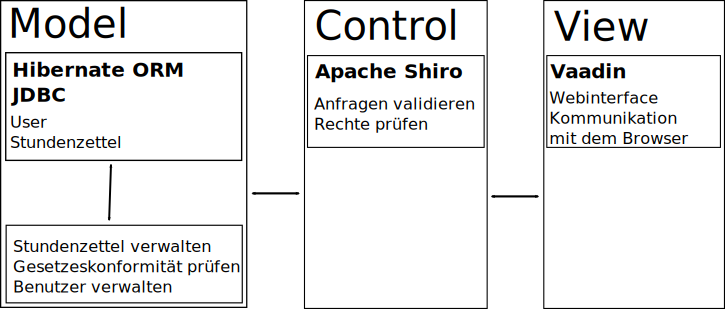
\includegraphics[width=\linewidth]{mvc.pdf}\\
\\
Die Architektur der Software basiert auf dem Model-View-Control (MVC) Modell, welches eine strikte Trennung von Daten/Logik (Model), Oberfläche (View) und Steuerung (Control) vorsieht.
Dies verbessert zum einen die Wartbarkeit und vereinfacht den Austausch einzelner Module, vor allem der Oberfläche.
\begin{itemize}
	\item \textbf{Model:}
		Das Model enthält die \emph{Benutzer*} und \emph{Stundenzettel}.
		Es enthält die Funktionalität um \emph{Benutzer*} und Stundenzettel zu verwalten.
		Außerdem prüft es, ob die \emph{Stundenzettel} den gesetzlichen Regelungen entsprechen und leitet sonst entsprechende Maßnahmen ein.
	\item \textbf{View:}
		Das View zeigt dem \emph{Benutzer*} alle Funktionalitäten und Informationen an, die für diesen relevant sind.
		Zudem nimmt es Befehle desselbigen entgegen.
		Es ist die Schnittstelle über die alle Interaktion mit dem \emph{Benutzer*} passiert.
	\item \textbf{Control:}
		Das Control prüft alle Anfragen die es vom View bekommt auf Korrektheit.
		Zudem prüft es ob der entsprechende \emph{Benutzer*} die nötigen Rechte für die Anfrage hat.
		Dann leitet es die Anfrage gegebenenfalls an das Model weiter.
\end{itemize}

	\section{Systemmodelle}

\includegraphics[width=\linewidth]{Anwendungsfalldiagramm.pdf}\\

	\section{Systemdesign}

\subsection{Login}
\includegraphics[width=\linewidth]{UI/Login/Login.png}

\newpage
\subsection{Benutzer*}

\textbf{\\Neue Zeiterfassung}\\
\\
Das ist die Hauptseite vom \emph{Benutzer*}, wo er direkt nach einer erfolgreichen Anmeldung oder durch Drücken auf die Schaltfläche "neue Zeiterfassung" landet. \\
Um eine neue Zeiterfassung zu starten, wählt der \emph{Benutzer*} eine Kategorie und eine Tätigkeit aus, anschließend drückt er auf Start Button. Der \emph{Benutzer*} kann die Zeiterfassung über das Stop Button beenden.\\
\\
\\
\includegraphics[width=\linewidth]{UI/Benutzer/Zeiterfassung.png}


\newpage
\textbf{\\Erfasste Zeiten bearbeiten}\\
\\
Das ist die Seite fürs Editieren der erfassten Zeiten vom \emph{Benutzer*}.
Man kann entweder direkt von der Seite "Neue Zeiterfassung" über das Edit Button \includegraphics[scale=.2]{UI/Button/Edit.png} oder durch auswählen vom Datum auf der Kalenderübersicht auf der linken Seite auf diese Seite landen. Nur die erfassten Zeiten, die noch nicht an den Betreuer abgegeben sind, könnten editiert werden.\\
Der \emph{Benutzer*} klickt in das Textfeld, wo er eine Änderung tätigen will, und ändert die dort eingetragene Daten. Anschließend klickt er auf das Save Button\includegraphics[scale=.2]{UI/Button/Save.png}, um die Änderungen zu bestätigen.\\
\\
\\
\includegraphics[width=\linewidth]{UI/Benutzer/Editieren.png}






\includegraphics[width=\linewidth]{UI/Benutzer/Nachricht.png}

\subsection{Betreuer}
\includegraphics[width=\linewidth]{UI/Betreuer/Hauptseite.png}\\
\includegraphics[width=\linewidth]{UI/Betreuer/Nachricht.png}

\subsection{Admin}
\includegraphics[width=\linewidth]{UI/Admin/Hauptseite.png}
\includegraphics[width=\linewidth]{UI/Admin/Accounts/Ubersicht.png}
\includegraphics[width=\linewidth]{UI/Admin/Accounts/Bearbeiten.png}

	\section{Glossar}
\begin{description}
	\item[Admin] Der Administrator. Höchste Entität, besitzt Rechte zum modizieren von angelegten Benutzern.
	               Erhält ebenfalls die eingesammelten Stundenzettel.

	\item[Stundenzettel] Formular auf dem die geleisteten Stunden mit Tätigkeit vermerkt werden.

	\item[Betreuer] Betreut mehrere Benutzer und kann deren Stundenzettel einsehen.
\end{description}


\end{document}
